\documentclass[a4paper, 10pt]{article}
\hyphenpenalty=8000
\textwidth=125mm
\textheight=185mm

\usepackage{graphicx}
\usepackage{float}
%this package is flexible for image insertion
%
\usepackage{alltt}
%this package is suitable for the description of algorithms and computer programs
%
\usepackage{amsmath}
%this package draws mathematical symbols smoothly
%
\usepackage[hidelinks, pdftex]{hyperref}
%this package produces hypertext links in the document

\pagenumbering{arabic}
\setcounter{page}{1}
\renewcommand{\thefootnote}{\fnsymbol{footnote}}
\newcommand{\doi}[1]{\href{https://doi.org/#1}{\texttt{https://doi.org/#1}}}

\begin{document}

\begin{center}
Nonlinear Analysis: Modelling and Control, Vol. vv, No. nn, YYYY\\
\copyright\ Vilnius University\\[24pt]
\LARGE
\textbf{Simulación de una escena en 2D}\\[6pt]
\small
\textbf {Camilo Alcocer, Harold Alfaro, Esteban Montero}\\[6pt]
IES "INFOTEP", Ciénaga Magdalena \\[6pt]
Received: 03/03/2025\quad/\quad
\end{center}

\begin{abstract}
Este informe presenta el desarrollo de un algoritmo en Python usando "Jupyter Notebook" para la simulación de una escena 2D, en la que un punto se desplaza sobre un rectángulo de fondo. \vskip 2mm

\textbf{Keywords:} Python, Jupyter Notebook, Simulación, 2D

\end{abstract}



\section{Introduction}\label{s:1}
En este informe se presenta el algoritmo que permite dibujar una escena en 2D sobre un rectangulo que contiene en su interior un punto, definiendo escenas que permiten dibujar, cambiar y actualizar el rectangulo, mediante el uso de Python. 

\section{Objetivos de la actividad}\label{s:2}
Dentro de los objetivos de la actividad está el familiarizarnos con las herramientas y sus interfaces, de este mismo modo entender el simulado de un objeto y poder manipular sus parámetros.

\section{Actividad}\label{s:2.1}
Este código define primero una clase "Escena" representando así el espacio 2D (Bidimensional) donde se dibujará el rectángulo y el punto dentro del mismo. 

\begin{figure}[ht]
\centering
\includegraphics[width=8.5cm]{image1.png}
\caption{Inicialización de la clase "Escena"}\label{fig:1}
\end{figure}

%
\raggedright 
A continuación, se establecen las funciones de nuestro algoritmo, como: "dibujar escena", "desplazar punto", "cambiar escena", "simular" y "actualizar".

\begin{figure}[H] % Usa [H] para fijar la posición
\centering
\includegraphics[width=8.5cm]{image2.png}

\vspace{0.5cm}

\includegraphics[width=8.5cm]{image3.png}

\vspace{0.5cm}

\includegraphics[width=8.5cm]{image4.png}

\vspace{0.5cm}

\includegraphics[width=8.5cm]{image5.png}
\caption{Definición de funciones}
\label{fig:1}
\end{figure}

\section{Resultados}\label{s:5}
Por último se definen los parámetros que imprimen el resultados de nuestras gráficas, ejmeplo:

\begin{figure}[H] % Usa [H] para fijar la posición
\centering
\includegraphics[width=8.5cm]{image6.png}
\caption{Imprimir resultados }
\label{fig:1}
\end{figure}

\subsection{Gráficas}
\vspace{0.5cm}

\begin{figure}[H] % Usa [H] para fijar la posición
\centering
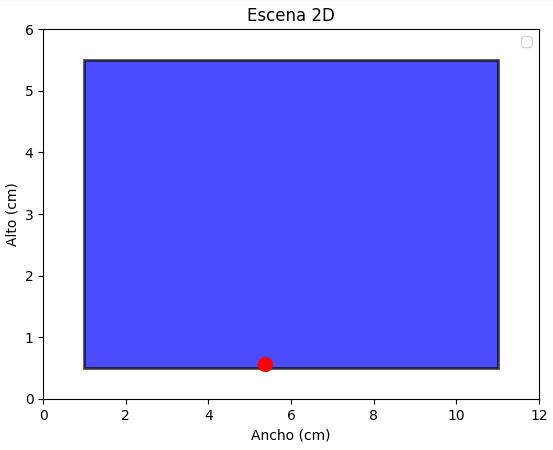
\includegraphics[width=8.5cm]{grafica1.png}
\caption{Primera gráfica con coordenadas [3,3]}
\label{fig:1}
\end{figure}

\begin{figure}[H] % Usa [H] para fijar la posición
\centering
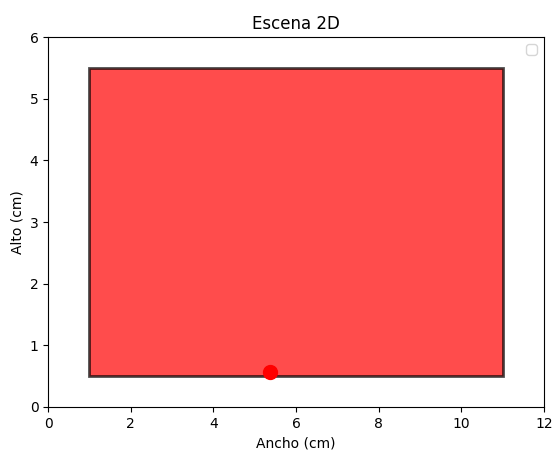
\includegraphics[width=8.5cm]{grafica2.png}
\caption{Segunda gráfica con coordenadas [5,5]}
\label{fig:1}
\end{figure}

\begin{figure}[H] % Usa [H] para fijar la posición
\centering
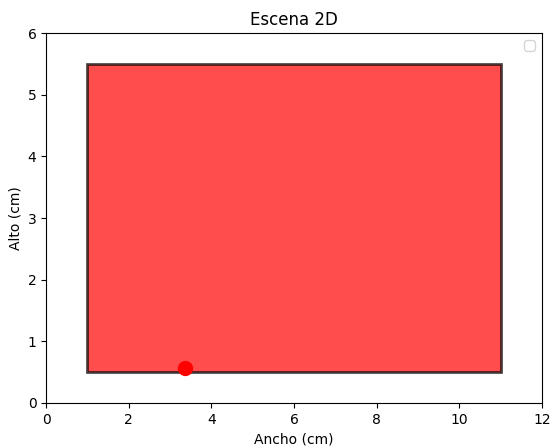
\includegraphics[width=8.5cm]{grafica3.png}
\caption{Tercera gráfica con coordenadas [5,5] ligeramente movida hacía la derecha}
\label{fig:1}
\end{figure}

\section{Conclusión}\label{s:5}
Finalmente, la actividad nos permitió poder familiarizarnos más con las interfaces de desarrollo, a su vez permite la retroalimentación de temas como programación orientada a objetos y Python. La simulación del punto que se desplaza en distintas direcciones según las medidas que le otorguemos permite tener conocimientos base de la materia. 

\end{document}
